\section{Base de données}

\subsection{Base de données d'utilisateurs}

Nous constituons une base de données d'utilisateur afin de stocker les utilisateurs ainsi que leurs données. Chaque utilisateur est identifié par un login et se connacte grace à ce login et un mot de passe. Dans la table est aussi entré un code représentant les droit de l'utilisateur, pour une question de sécurité. Chaque utilisateur peux posséder plusieurs fichier qui son stocké sur son répertoire dans le serveur. Ces fichiers sont aussi répertorié dans cette base de données.\\
\begin{figure}[position]
   \caption{Schéma de la base de données utilisateur}
   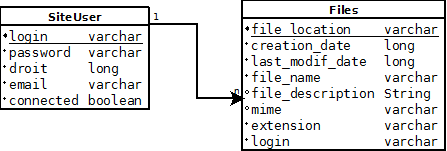
\includegraphics[scale=1]{BD1.png} 
\end{figure}


\subsection{Base de données de modules}

Nous constituons aussi une base de données de module permettant d'une part de recenser les différents module déployé sur le serveur, et d'autre part de permettre une génération dynamique des menus du site web en allant chercher directement dans la base de donnée les noms des liens ainsi que les pages à charger. Pour des raison de sécurité nous choisissons de ne pas proposer d'interface web pour l'ajout ou la suppression de données de cette base de données.\\
\begin{figure}[position]
   \caption{Schéma de la base de données utilisateur}
	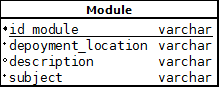
\includegraphics[scale=1]{DBmodule.png} 
\end{figure}